\documentclass[10pt,border=4pt]{standalone}
\usepackage{mathptmx}
\usepackage{amsmath,amssymb,bm}
\usepackage{tikz}
\usetikzlibrary{patterns,decorations.pathmorphing,decorations.pathreplacing,arrows.meta,fit,backgrounds,calc,positioning,shapes.geometric}
\definecolor{acc}{HTML}{0B5394}
\definecolor{accl}{HTML}{EAF0F7}
\definecolor{grp}{HTML}{F5F5F5}
\definecolor{org}{HTML}{C55A11}
\definecolor{orgl}{HTML}{FBEFE6}
\tikzset{
 dat/.style={draw=black,line width=0.6pt,fill=white,align=center,font=\small,inner sep=3pt,minimum height=0.85cm},
 lay/.style={draw=acc,line width=0.8pt,fill=accl,rounded corners=2pt,align=center,font=\small,inner sep=3pt,minimum height=0.85cm},
 cnd/.style={draw=org,line width=0.8pt,fill=orgl,rounded corners=2pt,align=center,font=\small,inner sep=3pt,minimum height=0.75cm},
 op/.style={circle,draw=black,line width=0.6pt,fill=white,inner sep=0.5pt,font=\small,minimum size=5mm},
 grpb/.style={draw=black!45,dashed,line width=0.6pt,rounded corners=3pt,inner sep=6pt},
 arr/.style={-{Latex[length=2.2mm,width=1.7mm]},line width=0.7pt},
 carr/.style={-{Latex[length=2.2mm,width=1.7mm]},line width=0.7pt,draw=org},
 shp/.style={font=\scriptsize,text=black!70,inner sep=1pt},
 lab/.style={font=\footnotesize,inner sep=1pt},
 ttl/.style={font=\small\bfseries,inner sep=0pt,anchor=west}
}
\newcommand{\xh}{\mathbf{x}_h}\newcommand{\xf}{\mathbf{x}_f}

\begin{document}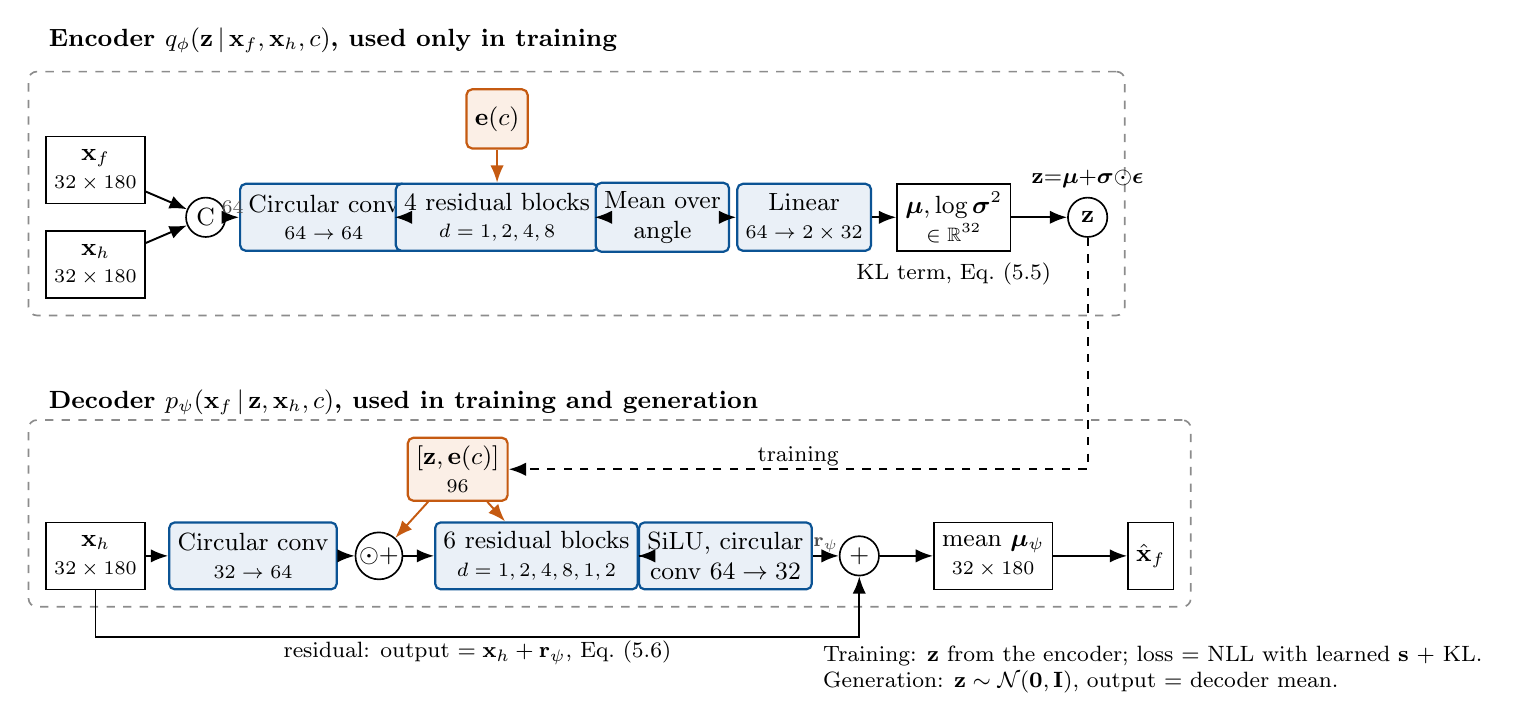
\begin{tikzpicture}[x=1cm,y=1cm]
\node[ttl] at (-0.6,2.25) {Encoder $q_\phi(\mathbf{z}\,|\,\xf,\xh,c)$, used only in training};
\node[dat] (xf) at (0,0.6) {$\xf$\\[-1pt]\scriptsize $32\times180$};
\node[dat] (xh) at (0,-0.6) {$\xh$\\[-1pt]\scriptsize $32\times180$};
\node[op] (cat) at (1.4,0) {C};
\node[lay] (s1) at (2.9,0) {Circular conv\\[-1pt]\scriptsize $64\to64$};
\node[lay] (b1) at (5.1,0) {4 residual blocks\\[-1pt]\scriptsize $d=1,2,4,8$};
\node[lay] (p1) at (7.2,0) {Mean over\\angle};
\node[lay] (l1) at (9.0,0) {Linear\\[-1pt]\scriptsize $64\to2\times32$};
\node[dat] (mu) at (10.9,0) {$\boldsymbol\mu,\log\boldsymbol\sigma^2$\\[-1pt]\scriptsize $\in\mathbb{R}^{32}$};
\node[op] (rp) at (12.6,0) {$\mathbf{z}$};
\draw[arr] (xf)--(cat); \draw[arr] (xh)--(cat); \draw[arr] (cat)--node[shp,above]{64}(s1); \draw[arr] (s1)--(b1); \draw[arr] (b1)--(p1); \draw[arr] (p1)--(l1); \draw[arr] (l1)--(mu); \draw[arr] (mu)--(rp);
\node[lab,above=2pt of rp] {$\mathbf{z}{=}\boldsymbol\mu{+}\boldsymbol\sigma{\odot}\boldsymbol\epsilon$};
\node[lab,below=3pt of mu] {KL term, Eq.~(5.5)};
\node[cnd] (e1) at (5.1,1.25) {$\mathbf{e}(c)$}; \draw[carr] (e1)--(b1);
\begin{scope}[on background layer]\node[grpb,fit=(xf)(xh)(rp)(e1)] (enc) {};\end{scope}
% decoder
\node[ttl] at (-0.6,-2.35) {Decoder $p_\psi(\xf\,|\,\mathbf{z},\xh,c)$, used in training and generation};
\node[dat] (xh2) at (0,-4.3) {$\xh$\\[-1pt]\scriptsize $32\times180$};
\node[lay] (s2) at (2.0,-4.3) {Circular conv\\[-1pt]\scriptsize $32\to64$};
\node[op] (f2) at (3.6,-4.3) {$\odot{+}$};
\node[lay] (b2) at (5.6,-4.3) {6 residual blocks\\[-1pt]\scriptsize $d=1,2,4,8,1,2$};
\node[lay] (o2) at (8.0,-4.3) {SiLU, circular\\conv $64\to32$};
\node[op] (ad) at (9.7,-4.3) {$+$};
\node[dat] (mean) at (11.4,-4.3) {mean $\boldsymbol\mu_\psi$\\[-1pt]\scriptsize $32\times180$};
\node[dat] (xg) at (13.4,-4.3) {$\hat{\mathbf{x}}_f$};
\draw[arr] (xh2)--(s2); \draw[arr] (s2)--(f2); \draw[arr] (f2)--(b2); \draw[arr] (b2)--(o2); \draw[arr] (o2)--node[shp,above]{$\mathbf{r}_\psi$}(ad); \draw[arr] (ad)--(mean); \draw[arr] (mean)--(xg);
\draw[arr] (xh2.south) -- ++(0,-0.6) -| node[lab,below,pos=0.25]{residual: output $=\xh+\mathbf{r}_\psi$, Eq.~(5.6)} (ad.south);
\node[cnd] (zc) at (4.6,-3.2) {$[\mathbf{z},\mathbf{e}(c)]$\\[-1pt]\scriptsize 96};
\draw[carr] (zc)--(f2); \draw[carr] (zc)--(b2);
\node[lab,align=left,anchor=north west] at (9.2,-5.4) {Training: $\mathbf{z}$ from the encoder; loss = NLL with learned $\mathbf{s}$ + KL.\\Generation: $\mathbf{z}\sim\mathcal{N}(\mathbf{0},\mathbf{I})$, output = decoder mean.};
\draw[arr,dashed] (rp.south) |- node[lab,above,pos=0.75]{training} (zc.east);
\begin{scope}[on background layer]\node[grpb,fit=(xh2)(xg)(zc)] (dec) {};\end{scope}
\end{tikzpicture}\end{document}
